% !TEX root = ../main.tex
% 本文件由 build-tex.sh 从 24-DSP指南-第24章中译.md 生成，改内容请改 md 后重新生成

\chapter{线性图像处理}\label{ch-24}

线性图像处理(linear image processing)基于与常规 DSP
相同的两种技术：卷积和傅里叶分析。两者中卷积更重要，因为图像的信息编码在空间域(spatial
domain)而不是频域里。线性滤波能从许多方面改善图像：锐化物体的边缘、降低随机噪声、校正不均匀的照明、用去卷积(deconvolution)校正模糊和运动等。这些处理都是把原图像与一个合适的滤波器核卷积，得到滤波后的图像。图像卷积的一个严重问题是需要进行的计算量巨大，执行时间常常长得无法接受。本章介绍为各种图像处理任务设计滤波器核的策略，还介绍两种缩短执行时间的重要技术：可分离卷积(convolution
by separability)和 FFT 卷积。

\section{卷积}

图像卷积的原理和一维卷积一样。例如，图像可以看作许多冲激之和，即经过缩放和平移的冲激函数。同样，线性系统由它对冲激的响应来刻画，也就是它的冲激响应。不出所料，系统的输出图像等于输入图像与系统冲激响应的卷积。

二维冲激函数是这样一幅图像：除了位于第 0 行、第 0 列的一个像素值为 1
外，其余全为零。暂且假定行、列下标都可以取正值和负值，使这个 1
位于一片零的汪洋正中。冲激函数通过线性系统后，这个唯一的非零点会变成另一种二维图案。由于一个点能发生的唯一变化就是扩散开来，图像处理的行话里常把冲激响应叫做点扩散函数(point
spread function，PSF)。

人眼是说明这些概念的绝佳例子。上一章讲过，视网膜第一层把以光的图案表示的图像，转换成以神经冲动图案表示的图像。视网膜第二层处理这幅神经图像，再把它传给第三层，也就是构成视神经的纤维。设想投射到视网膜上的图像，是暗背景正中的一个很小的光点，也就是给眼睛输入了一个冲激。假定这个系统是线性的，那么观察出现在视神经上的图像，就能确定视网膜里进行的图像处理。换句话说，我们要找出这个处理过程的点扩散函数。本章后面还会回来讨论''眼睛是线性的''这个假设。

图 24-1 概括了这个实验。(a) 表示打到视网膜上的冲激，(b)
表示出现在视神经上的图像。中间层让明亮的尖峰通过，但在它周围产生一圈更暗的区域。眼睛是通过一种叫侧抑制(lateral
inhibition)的过程做到这一点的：中间层的一个神经细胞被激活时，会降低它附近邻居被激活的能力。眼睛观看一幅完整的图像时，图像中的每个点都向视神经上的图像贡献一个经过缩放和平移的冲激响应。换句话说，看到的图像与这个
PSF 卷积，产生传给大脑的神经图像。显而易见的问题是：把看到的图像与这个
PSF 卷积，怎么就能提高眼睛理解世界的能力？

\begin{figure}[htbp]
\centering
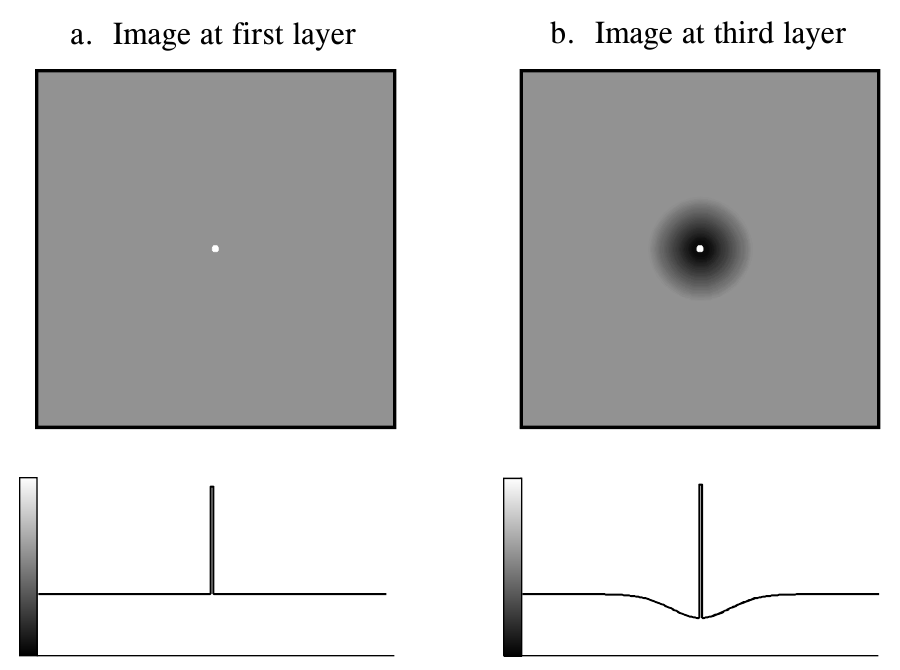
\includegraphics[width=0.750\linewidth,height=0.8\textheight,keepaspectratio]{assets/ch24/fig24-01.png}
\caption*{\textbf{图 24-1　眼睛的 PSF。} 视网膜中间层把 (a) 所示的冲激，变成 (b)
所示的、周围有一圈暗区的冲激。这个点扩散函数增强了物体的边缘。 （a.
Image at first layer = 第一层的图像；b. Image at third layer =
第三层的图像。下方曲线是穿过图像中心的亮度剖面，左侧灰度条表示亮度刻度。）}
\end{figure}

人和其他动物用视觉识别附近的物体，比如敌人、食物和配偶。这是靠根据亮度和颜色的差异，把图像中的一个区域与另一个区域区分开来做到的。换句话说，识别物体的第一步是找出它的边缘，也就是把物体与背景分开的那条不连续处。视网膜中间层通过锐化所见图像中的边缘来帮助完成这项任务。为了说明它的作用，图
24-2 给出一幅由暗缓慢过渡到亮的图像，它的边缘模糊、不清晰。(a)
是这幅图像的强度剖面，即进入眼睛的亮度分布。(b)
是出现在视神经上的亮度剖面，即传给大脑的图像。视网膜里的处理使明暗区域之间的边缘显得更陡峭，强化了''这两个区域不同''的印象。

\begin{figure}[htbp]
\centering
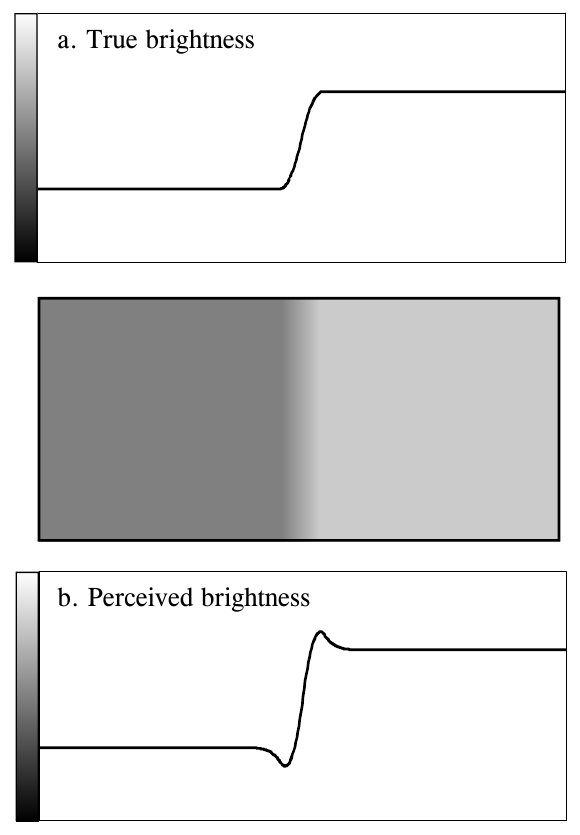
\includegraphics[width=0.483\linewidth,height=0.8\textheight,keepaspectratio]{assets/ch24/fig24-02.png}
\caption*{\textbf{图 24-2　马赫带。} 视网膜中的图像处理使 (a)
那样缓慢变化的边缘被锐化成 (b)
那样。这使图像中的物体更容易分开，但会产生一种叫马赫带(Mach
bands)的视错觉：在边缘附近，过冲使暗区显得更暗、亮区显得更亮，从而产生平行于边缘的暗带和亮带。
（a. True brightness = 真实亮度；b. Perceived brightness =
感知到的亮度。中间的灰度图是这条边缘本身。）}
\end{figure}

边缘响应中的过冲(overshoot)造成了一种有趣的视错觉。紧挨边缘处，暗区显得格外暗，亮区显得格外亮。由此形成的明暗条带叫马赫带，以首先描述它的奥地利物理学家恩斯特·马赫（Ernst
Mach，1838--1916）命名。

和一维信号一样，图像卷积也可以从两个角度来看：从输入端看和从输出端看。从输入端看，输入图像中的每个像素都向输出图像贡献一个经过缩放和平移的点扩散函数。从输出端看，输出图像中的每个像素都受输入信号中一组像素的影响。对一维信号，这个影响区域就是左右翻转后的冲激响应；对图像信号，它是左右翻转并上下翻转后的
PSF。由于 DSP 中用的大多数 PSF
关于竖直轴和水平轴都对称，这些翻转不起作用，可以忽略。本章后面会看到一些不对称的
PSF，就必须考虑翻转了。

图 24-3 给出了几种常见的 PSF。(a)
中的圆柱(pillbox)顶面是圆的，侧面是直的。例如，如果相机镜头没有对准焦，图像中的每个点都会投射成图像传感器上的一个圆斑（回头看图
23-2，想想把投影屏移近或移远镜头会怎样）。换句话说，圆柱就是失焦镜头的点扩散函数。

\begin{enumerate}
\def\labelenumi{(\alph{enumi})}
\setcounter{enumi}{1}
\tightlist
\item
  中的高斯是受随机缺陷限制的成像系统的
  PSF。例如，望远镜的图像会被大气湍流弄模糊，使每个光点在最终图像中都变成一个高斯。CCD
  和视网膜这类图像传感器，常常受光和/或电子散射的限制。中心极限定理表明，这类随机过程造成的就是高斯模糊。
\end{enumerate}

圆柱和高斯在图像处理中的用法，就像一维信号中的移动平均滤波器。图像与这些
PSF
卷积后会显得模糊、边缘不那么清晰，但随机噪声更低。从它们在时域（空间域）的作用看，这类滤波器叫平滑滤波器(smoothing
filter)；从它们对频域的处理看，叫低通滤波器。(c) 中的方形 PSF
也可以用作平滑滤波器，但它不是圆对称的，导致对角方向的模糊程度与竖直、水平方向不同。这一点重要与否，取决于具体用途。

平滑滤波器的反面是边缘增强(edge enhancement)滤波器，也就是高通滤波器。第
14 章讨论的频谱反转(spectral inversion)技术用于在两者之间转换。如 (d)
所示，边缘增强滤波器核是取平滑滤波器的负值，再在中心加一个冲激函数构成的。视网膜里进行的图像处理就是这类滤波器的一个例子。

\begin{enumerate}
\def\labelenumi{(\alph{enumi})}
\setcounter{enumi}{4}
\tightlist
\item
  是二维 sinc 函数。一维信号处理用加窗 sinc
  来分离频带。由于图像的信息不编码在频域，sinc
  函数很少用作图像滤波器核，不过在一些理论问题中确实用得到。sinc
  函数可能不好用，因为它的尾部幅度衰减得很慢（按
  \(1/x\)），这意味着必须把它当作无限宽来对待。相比之下，高斯的尾部衰减得非常快（按
  \(e^{-x^2}\)），最终可以截断而不造成不良影响。
\end{enumerate}

\begin{figure}[htbp]
\centering
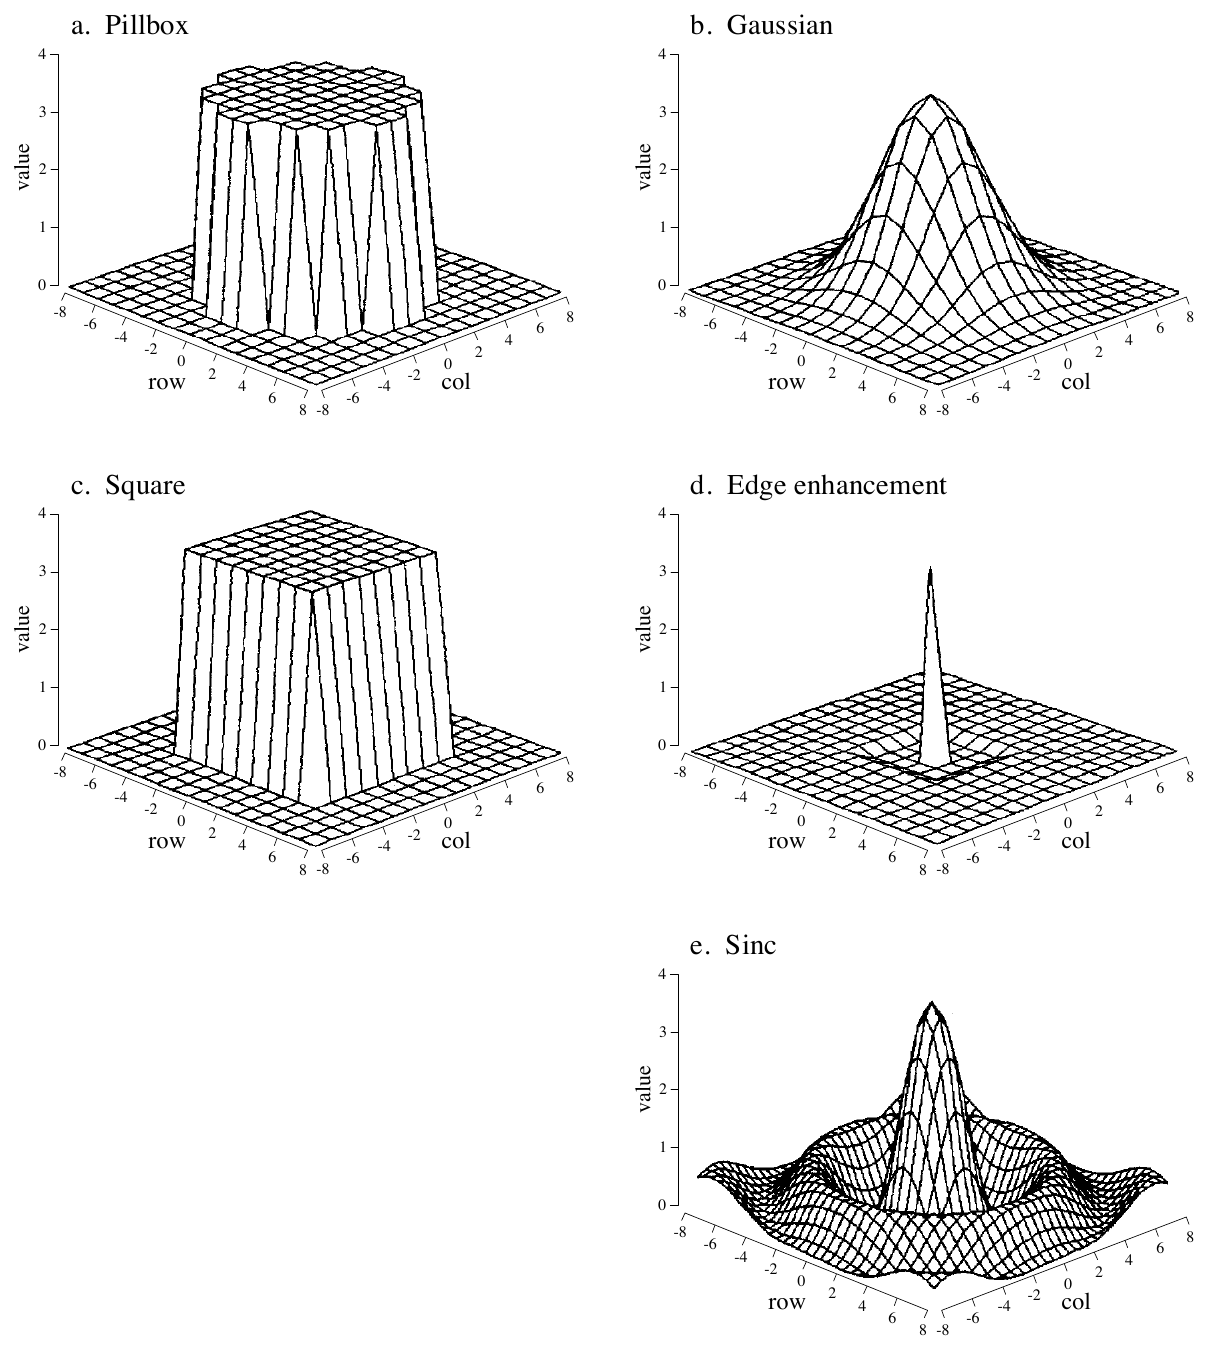
\includegraphics[width=1.000\linewidth,height=0.8\textheight,keepaspectratio]{assets/ch24/fig24-03.png}
\caption*{\textbf{图 24-3　常见的点扩散函数。} (a)、(b)、(c)
所示的圆柱、高斯和方形是常见的平滑（低通）滤波器。如 (d)
所示，从冲激中减去低通核，就得到边缘增强（高通）滤波器。(e) 中的 sinc
函数在图像处理中用得很少，因为图像的信息编码在空间域而不是频域。 （a.
Pillbox = 圆柱；b. Gaussian = 高斯；c.~Square = 方形；d.~Edge
enhancement = 边缘增强；e. Sinc = sinc 函数。value = 值，row = 行，col =
列。原书图注排在 (e) 左侧，已去掉，译文见上。）}
\end{figure}

所有这些滤波器核在行和列上都使用负下标，使 PSF 能以第 0 行、第 0
列为中心。在一维 DSP
中，常常把滤波器核向右平移，直到所有非零采样都有正下标，从而消除负下标。这种平移会使输出信号移动同样的量，通常无关紧要。相比之下，输入图像和输出图像之间出现平移，一般是不可接受的。因此，图像处理中的滤波器核用负下标是常态。

图像卷积的一个问题是计算量很大。例如，一幅 512×512 像素的图像与一个
64×64 像素的 PSF 卷积，需要超过十亿次乘法和加法（即
64×64×512×512）。漫长的执行时间可能使这些技术不实用。有三种方法可以提速。

第一种策略是使用非常小的 PSF，常常只有 3×3
像素。做法是遍历输出图像的每个采样，用优化过的代码把输入图像中对应的九个像素相乘并累加。仅仅一个
3×3 的 PSF 就能完成数量惊人的处理，因为它的大小足以影响图像中的边缘。

第二种策略用在需要大
PSF、但对它的形状要求不严的场合。这要求滤波器核是可分离的(separable)，这种性质使图像卷积可以通过一系列一维运算来完成，能把执行速度提高数百倍。

第三种策略是 FFT
卷积，用在滤波器核很大、并且有特定形状的场合。即使有高效的 FFT
带来的提速，执行时间也会长得吓人。下面详细看看这三种策略，以及它们在图像处理中的应用实例。

\section{3×3 边缘修饰}

图 24-4 给出了几种 3×3 运算。(a) 是机场 X
光行李扫描仪采集的一幅图像。这幅图像与 3×3 冲激函数（一个 1 周围是 8 个
0）卷积后保持不变。这本身没什么意思，但它是其他滤波器核的基准。

\begin{enumerate}
\def\labelenumi{(\alph{enumi})}
\setcounter{enumi}{1}
\item
  是图像与一个由一个 1、一个 −1 和 7 个 0 组成的 3×3
  核卷积的结果。这叫平移相减(shift and
  subtract)运算，因为是从原图像（对应那个
  1）中减去图像的一个平移版本（对应那个
  −1）。这种处理产生一种视错觉：有些物体看起来比背景更近或更远，形成立体或浮雕效果。大脑解读图像时，假定光是从上方照来的，这是世界通常呈现给我们的样子。如果一个物体的边缘上亮下暗，它就被感知为从背景中凸出来。再看一个有趣的效果：把图片倒过来，物体就会陷进背景里。
\item
  给出了一个边缘检测(edge detection) PSF
  和得到的图像。原图像中的每条边缘都被变换成平行于原边缘的窄暗带和窄亮带。对这幅图像做阈值处理，可以分离出暗带或亮带，从而得到一种检测图像边缘的简单算法。
\end{enumerate}

\begin{figure}[htbp]
\centering
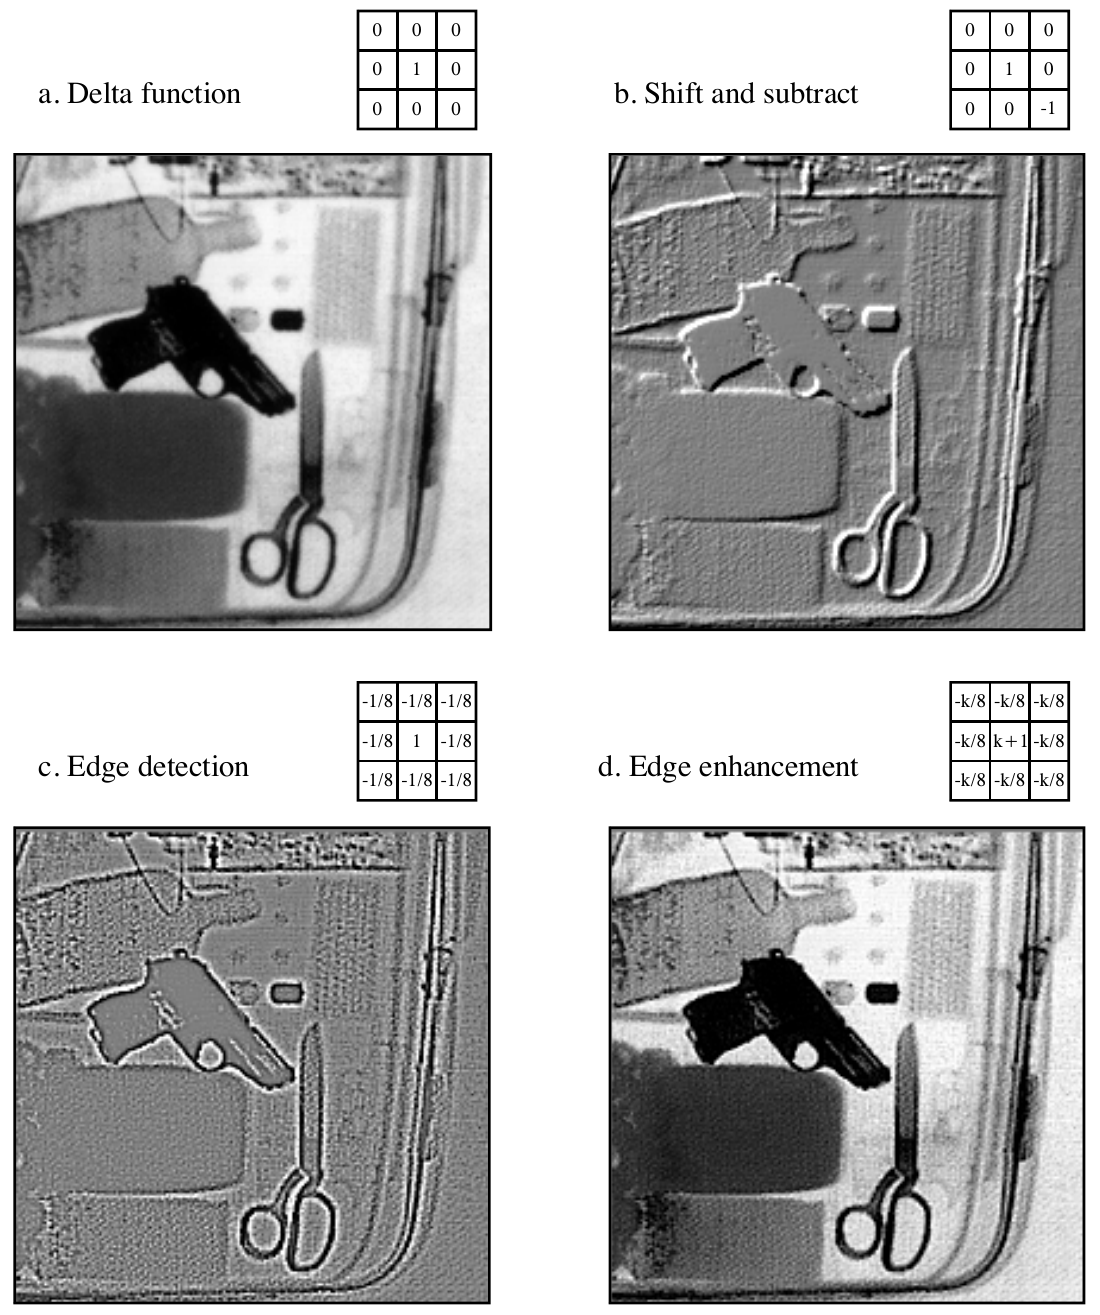
\includegraphics[width=0.917\linewidth,height=0.8\textheight,keepaspectratio]{assets/ch24/fig24-04.png}
\caption*{\textbf{图 24-4　3×3 边缘修饰。} 原图像 (a) 是在机场 X
光行李扫描仪上采集的。(b) 所示的平移相减运算产生一种伪三维效果。(c)
中的边缘检测算子去除了全部对比度，只留下边缘信息。(d)
中的边缘增强滤波器把 (a) 和 (c) 两幅图像按不同比例相加，比例由参数 k
决定。这幅图用的是 k = 2。 （a. Delta function = 冲激函数；b. Shift and
subtract = 平移相减；c.~Edge detection = 边缘检测；d.~Edge enhancement =
边缘增强。每个子图右上角的 3×3 方格是所用的核。）}
\end{figure}

\begin{enumerate}
\def\labelenumi{(\alph{enumi})}
\setcounter{enumi}{3}
\tightlist
\item
  展示了一种常用的图像处理技术：边缘增强，有时也叫锐化(sharpening)运算。在
  (a) 中，物体的对比度(contrast)很好（明暗程度合适），但边缘非常模糊。在
  (c)
  中，物体完全没有对比度，但边缘非常锐利。策略是把边缘好的那幅图像乘以一个常数
  k，再加到对比度好的那幅图像上。这等价于把原图像与 (d) 所示的 3×3 PSF
  卷积。如果 k 取 0，这个 PSF 就变成冲激函数，图像保持不变。k
  越大，图像的边缘越清晰。(d) 中的图像用的是 k = 2：两份图像 (c)
  加一份图像
  (a)。这种运算模仿了眼睛锐化边缘的能力，让物体更容易从背景中分离出来。
\end{enumerate}

与这些 PSF
中的任何一个卷积，都可能使最终图像出现负的像素值。即使程序能处理负像素值，图像显示器也不能。最常用的解决办法是给每个算出的像素加一个偏移量，这几幅图就是这样做的。另一种办法是截掉超出范围的值。

\section{可分离卷积}

只要 PSF 是可分离的，这就是一种快速卷积技术。如果一个 PSF
能分解成两个一维信号------一个竖直投影和一个水平投影------就称它是可分离的。图
24-5 是可分离图像的一个例子：方形
PSF。具体地说，图像中每个像素的值，等于水平投影中对应的点乘以竖直投影中对应的点。写成数学式：

\textbf{公式
24-1}　图像分离。如果一幅图像能分解成水平和竖直投影，就称它是可分离的。

\[x[r,c] = \text{vert}[r] \times \text{horz}[c]\]

其中 x{[}r, c{]} 是二维图像，vert{[}r{]} 和 horz{[}c{]}
是一维投影。显然，大多数图像不满足这个要求，例如圆柱就不可分离。不过，可分离的图像有无穷多个。这一点可以这样理解：随意生成水平和竖直投影，再找出与之对应的图像。例如，图
24-6 用双边指数(double-sided
exponential)剖面说明了这一点。与这些剖面对应的图像再由公式 24-1
求出。显示出来，这幅图像呈菱形，随着离原点的距离增大按指数衰减到零。

\begin{figure}[htbp]
\centering
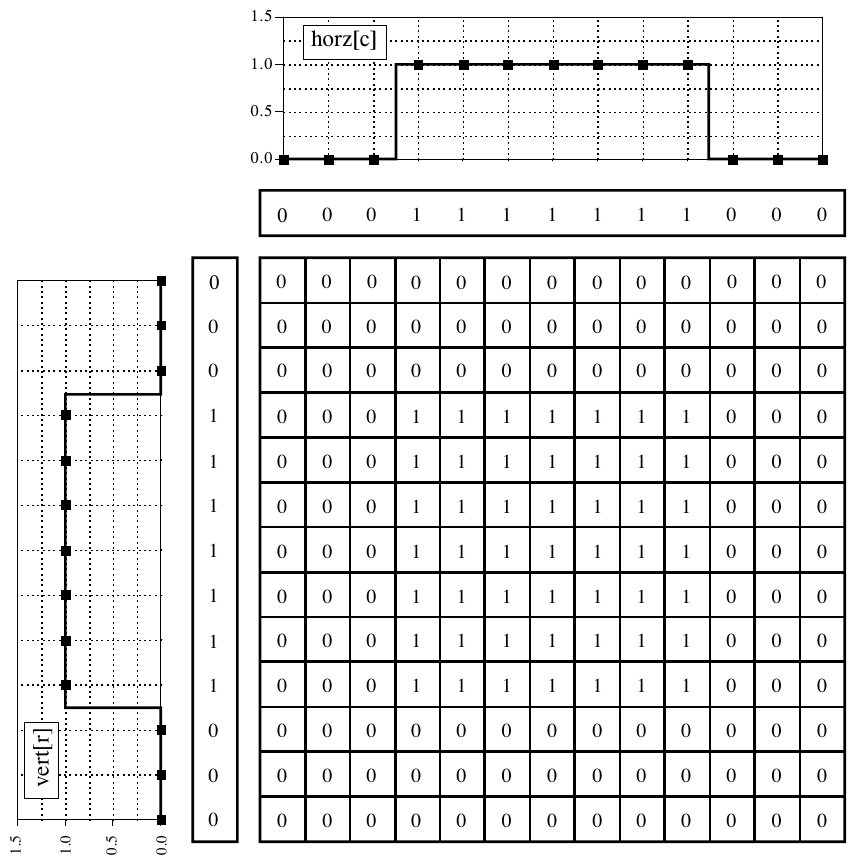
\includegraphics[width=0.713\linewidth,height=0.8\textheight,keepaspectratio]{assets/ch24/fig24-05.png}
\caption*{\textbf{图 24-5　矩形 PSF 的分离。} 如果一个 PSF
能分解成水平和竖直剖面，就称它是可分离的。可分离的 PSF
很重要，因为它们能被快速卷积。 （horz{[}c{]} = 水平投影，vert{[}r{]} =
竖直投影。原书图注排在左上，已去掉，译文见上。）}
\end{figure}

\begin{figure}[htbp]
\centering
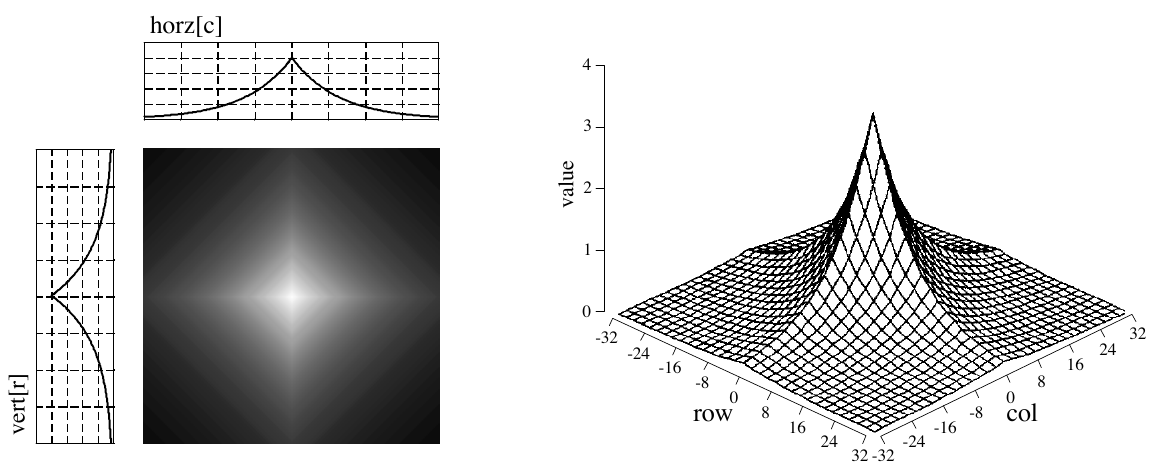
\includegraphics[width=0.963\linewidth,height=0.8\textheight,keepaspectratio]{assets/ch24/fig24-06.png}
\caption*{\textbf{图 24-6　构造可分离的 PSF。}
先任意定义投影，再计算与之对应的二维函数，就能生成无穷多个可分离的
PSF。本例中两个剖面都选为双边指数，得到菱形的 PSF。 （horz{[}c{]} =
水平投影，vert{[}r{]} = 竖直投影；右边三维图中 value = 值，row = 行，col
= 列。）}
\end{figure}

在大多数图像处理任务中，理想的 PSF
是圆对称的，比如圆柱。尽管数字图像通常以行和列的矩形格式存储和处理，人们还是希望在所有方向上对图像做同样的修改。这就引出一个问题：有没有既圆对称又可分离的
PSF？答案是有，但只有一个：高斯。如图 24-7
所示，二维高斯图像的投影也是高斯。图像高斯和投影高斯的标准差相同。

\begin{figure}[htbp]
\centering
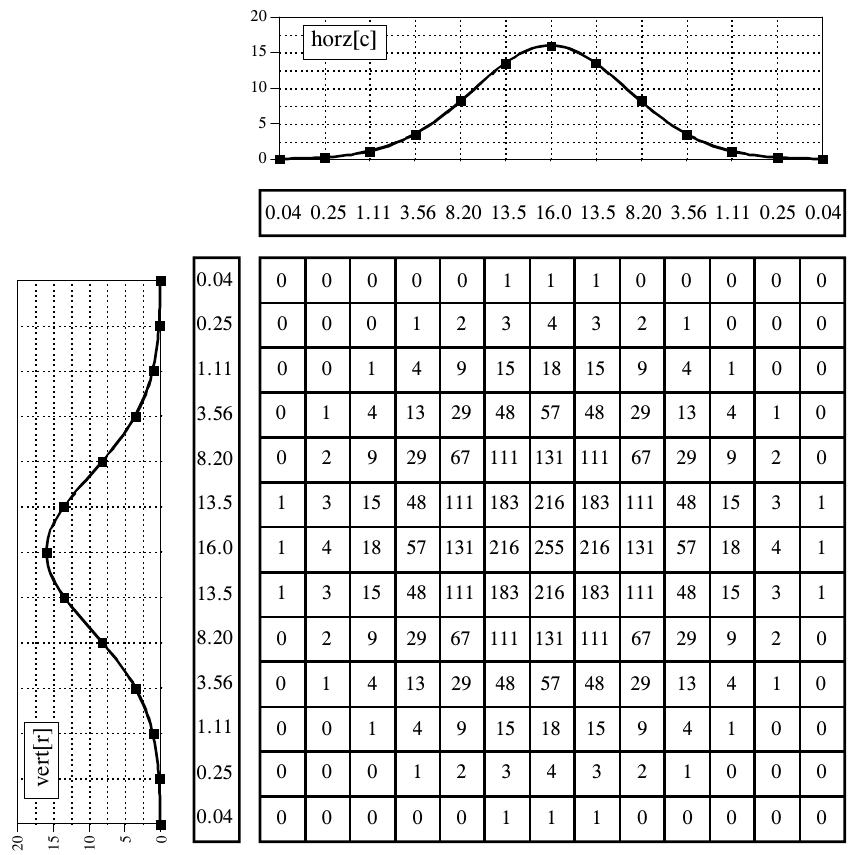
\includegraphics[width=0.713\linewidth,height=0.8\textheight,keepaspectratio]{assets/ch24/fig24-07.png}
\caption*{\textbf{图 24-7　高斯的分离。} 高斯是唯一既圆对称又可分离的
PSF。这使它成为图像处理中常用的滤波器核。 （horz{[}c{]} =
水平投影，vert{[}r{]} = 竖直投影。原书图注排在左上，已去掉，译文见上。）}
\end{figure}

要把图像与可分离的滤波器核卷积，先把图像的每一行与水平投影卷积，得到一幅中间图像；再把这幅中间图像的每一列与
PSF
的竖直投影卷积。所得图像与原图像和滤波器核直接卷积的结果完全相同。如果你愿意，也可以先卷列再卷行，结果一样。

N×N 的图像与 M×M 的滤波器核卷积，所需时间与 \(N^2M^2\)
成正比。换句话说，输出图像的每个像素都依赖于滤波器核中的所有像素。相比之下，可分离卷积只需要与
\(N^2M\)
成正比的时间。对于几百个像素宽的滤波器核，这种技术能把执行时间缩短几百倍。

还可以更好。如果你愿意使用矩形 PSF（图 24-5）或双边指数 PSF（图
24-6），计算效率还会更高。这是因为对应的一维卷积分别是移动平均滤波器（第
15 章）和双向单极点滤波器(bidirectional single pole filter，第 19
章）。这两种一维滤波器都能用递归快速实现。这样一来，图像卷积的时间只与
\(N^2\) 成正比，完全与 PSF 的大小无关。换句话说，图像可以与任意大的 PSF
卷积，每个像素只需几次整数运算。例如，在个人计算机上卷积一幅 512×512
的图像只需几百毫秒。真快！不喜欢这两种滤波器核的形状？那就把图像与其中一种卷积几次，近似出高斯
PSF（由第 7
章的中心极限定理保证）。这些都是很棒的算法，能在失败的边缘把成功抢回来，非常值得记住。

\section{大 PSF 的例子：照明平坦化}

需要大 PSF
的一个常见应用，是增强照明不均匀的图像。可分离卷积是完成这种处理的理想算法。除少数例外，眼睛看到的图像都是由反射光形成的。这意味着看到的图像等于物体的反射率(reflectance)乘以环境照明(illumination)。图
24-8 说明了这一点。(a) 代表所看场景的反射率，这里是一系列明暗条纹。(b)
是一个照明信号的例子，即落在 (a)
上的光的分布。和真实世界一样，照明在成像区域上缓慢变化。(c)
是眼睛看到的图像，等于反射率图像 (a) 乘以照明图像 (b)。(c)
中照明差的区域很难看清，原因有二：太暗，而且对比度（峰与谷之差）太低。

为了理解这和日常视觉问题有什么关系，设想你在看两个穿着完全相同的人，一个站在明亮的阳光下，另一个站在附近一棵树的树荫里。两人反射入射光的百分比相同，比如脸反射
80\%，灰衬衫反射 40\%，深色裤子反射
5\%。问题是，两人受到的照明可能相差比如十倍。这使树荫里那人的图像比阳光下的人暗十倍，（脸、衬衫和裤子之间的）对比度也小十倍。

图像处理的目标是把采集到的图像中的照明分量弄平。换句话说，我们希望最终图像代表的是物体的反射率，而不是光照条件。用图
24-8 的话说，就是已知 (c)，求
(a)。这是一个非线性滤波问题，因为两个分量图像是相乘而不是相加组合在一起的。虽然这种分离无法做到完美，改善却可能非常显著。

首先，我们把图像 (c) 与一个大 PSF 卷积，PSF
的大小是整幅图像的五分之一。目的是消除 (c) 中的锐利特征，得到原照明信号
(b) 的一个近似。这里就要用到可分离卷积。PSF
的确切形状并不重要，只要它比反射率图像中的特征宽得多就行。(d)
是用高斯滤波器核得到的结果。

既然平滑滤波器给出了照明图像的估计，我们就用边缘增强滤波器来求反射率图像。也就是把图像
(c)
与''冲激函数减去高斯''构成的滤波器核卷积。为了缩短执行时间，做法是从原图像
(c) 中减去平滑后的图像 (d)。(e)
是结果。行不通！暗区虽然被适当提亮了，但这些区域的对比度仍然很差。

线性滤波在这个应用中表现很差，因为反射率信号和照明信号原本是相乘而不是相加组合的。线性滤波无法正确分离通过非线性运算组合的信号。要分离这些信号，必须把它们''解乘''。换句话说，应该用原图像除以平滑后的图像，如
(f) 所示。这样既校正了亮度，又把对比度恢复到了合适的水平。

\begin{figure}[htbp]
\centering
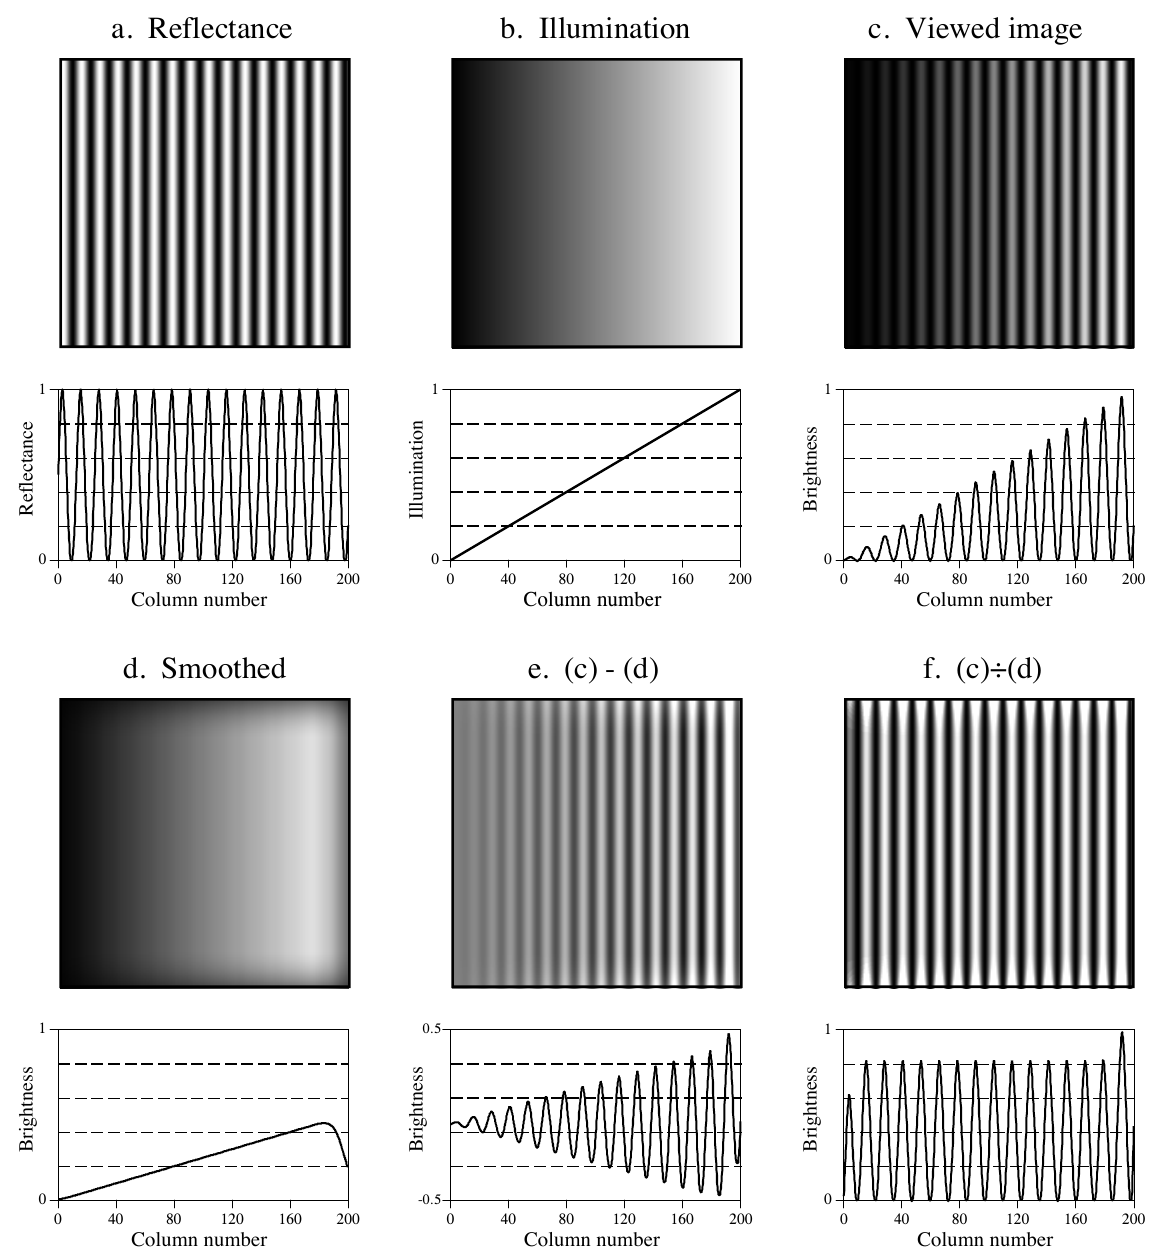
\includegraphics[width=0.958\linewidth,height=0.8\textheight,keepaspectratio]{assets/ch24/fig24-08.png}
\caption*{\textbf{图 24-8　成像模型。}（上半部分）看到的图像 (c) 由照明图案 (b)
乘以反射率图案 (a) 得到。图像处理的目标是修改 (c)，使它看起来更像
(a)。这在 (d)、(e)、(f) 中完成。（下半部分，原书为下一页的''图
24-8（续）``）(d) 是 (c) 的平滑版本，用作照明信号的近似。(e)
是用看到的图像减去平滑图像得到的反射率图像近似。(f)
是用两幅图像相除这一非线性过程得到的更好的近似。 （a. Reflectance =
反射率；b. Illumination = 照明；c.~Viewed image =
看到的图像；d.~Smoothed = 平滑后；e. (c) − (d)；f.~(c) ÷ (d)。Brightness
= 亮度，Column number = 列号。原书 (a)～(c) 和 (d)～(f)
分在两页，这里上下拼成一张。）}
\end{figure}

这种图像相除的做法与同态处理(homomorphic processing)密切相关，后者在第
22
章介绍过。同态处理是处理通过非线性运算组合的信号的一种方法。策略是通过适当的数学运算，把非线性问题变成线性问题。两个信号通过乘法组合时，同态处理先对采集到的信号取对数。利用恒等式
\(\log(a \times b) = \log(a) + \log(b)\)，分离相乘信号的问题就转化成了分离相加信号的问题。例如，对图像
(c)
取对数后，可以用一个线性高通滤波器分离出反射率图像的对数。和前面一样，实现高通滤波最快的办法是减去图像的平滑版本。然后用反对数（指数）撤销对数，就得到所要的反射率图像近似。

相除和走同态路线，哪个更好？两者几乎一样，因为取对数后相减就等于相除。唯一的区别在于照明图像的近似：一种方法用采集图像的平滑版本，另一种用采集图像对数的平滑版本。

这种照明平坦化技术非常有用，以至于被纳入了眼睛的神经结构。前面把视网膜中间层的处理描述为边缘增强或高通滤波器。这没错，但不是全部。眼睛的第一层是非线性的，大致是对进来的图像取对数。这使眼睛成为一个同态处理器。正如上面所说，对数之后接一个线性边缘增强滤波器，就能把照明分量弄平，让眼睛在光照条件差的情况下也能看清。同态处理的另一个有趣应用出现在摄影中：底片的密度（黑度）等于最终照片亮度的对数。这意味着冲洗阶段对底片的任何处理，都是一种同态处理。

讲完这个例子之前，还有一件麻烦事需要提一下。第 6 章讲过，N 点的信号与 M
点的滤波器核卷积，得到的信号长 N+M−1 点。同样，M×M 的图像与 N×N
的滤波器核卷积，结果是 (M+N−1)×(M+N−1)
的图像。问题是，图像尺寸变来变去往往很难处理。例如，分配的内存要变，视频显示要调整，数组下标可能也要改。常见的处理办法是不管它：如果开始是
512×512 的图像，我们希望最后得到的也是 512×512
的图像。超出原边界的像素被丢弃。

这虽然保持了图像大小，却没有解决全部问题：卷积还有边界条件(boundary
condition)的问题。例如，设想计算 (d) 右上角的那个像素。做法是把高斯 PSF
的中心放在 (c) 的右上角上，然后把 (c) 中的每个像素与覆盖在上面的 PSF
中对应的像素相乘，再把乘积相加。问题是 PSF
有四分之三落在已定义的图像之外。最简单的做法是把这些未定义的像素赋值为零。(d)
就是这样做出来的，这也是图像四周出现一圈暗带的原因：亮度向已定义图像之外的零像素值平滑下降。

幸好，边框周围的这圈暗区是可以校正的（虽然这个例子没有校正）。做法是把
(d) 中的每个像素除以一个校正因子。校正因子是计算该像素时 PSF
浸没在输入图像中的比例。也就是说，要校正 (d) 中的某个像素，设想 PSF 以
(c) 中对应的像素为中心。例如，(c) 的右上角像素只有 25\% 的 PSF
与输入图像重叠，因此把 (d) 中这个像素除以 0.25 来校正。这意味着 (d)
中心的像素不会改变，而四周的暗像素会被提亮。要求出校正因子，可以设想把滤波器核与一幅所有像素值都为
1 的图像卷积，所得图像中的像素就是消除边缘效应所需的校正因子。

\section{傅里叶图像分析}

傅里叶分析在图像处理中的用法与一维信号大致相同。不过，图像的信息不编码在频域，这使这些技术的用处小得多。例如，对音频信号做傅里叶变换，令人困惑的时域波形就变成了易于理解的频谱。相比之下，对图像做傅里叶变换，却把空间域中直截了当的信息变成了频域中一团乱麻。简言之，别指望傅里叶变换帮你理解图像中编码的信息。

同样，也别指望在频域中设计滤波器。图像的基本特征是边缘，即把一个物体或区域与另一个物体或区域分开的线。由于边缘由很宽范围的频率成分组成，试图通过操纵频谱来修改图像，通常没什么成效。图像滤波器一般在空间域中设计，信息在那里以最简单的形式编码。要从平滑和边缘增强运算（空间域）的角度去想，而不是从高通和低通滤波器（频域）的角度去想。

尽管如此，傅里叶图像分析确实有几个有用的性质。例如，空间域中的卷积对应频域中的乘法。这很重要，因为乘法是比卷积简单的数学运算。和一维信号一样，这个性质使
FFT
卷积和各种去卷积技术成为可能。频域的另一个有用性质是傅里叶切片定理(Fourier
Slice
Theorem)，即一幅图像与它的投影（从侧面看这幅图像）之间的关系。这是计算机断层扫描(computed
tomography)的基础，这种 X 光成像技术广泛用于医学和工业。

图像的频谱可以用几种方法计算，但这里介绍的 FFT
方法是唯一实用的。原图像必须由 N 行 × N 列组成，N 是 2 的幂，即
256、512、1024 等。如果原图像的大小不是 2
的幂，就补上值为零的像素，使它达到合适的大小。我们把存放图像的二维数组叫做实部数组。此外还需要一个同样大小的数组，叫做虚部数组。

计算图像傅里叶变换的方法很简单：先对每一行做一维 FFT，再对每一列做一维
FFT。具体地说，先对实部数组第 0 行的 N 个像素值做 FFT。FFT
输出的实部放回实部数组的第 0 行，虚部放进虚部数组的第 0 行。对第 1 到第
N−1
行重复这个过程后，实部和虚部数组中都是一幅中间图像。接着，对中间数据的每一列重复这个过程：取实部数组第
0 列的 N 个像素值和虚部数组第 0 列的 N 个像素值，计算 FFT。FFT
输出的实部放回实部数组的第 0 列，虚部放回虚部数组的第 0 列。对第 1 到第
N−1 列重复后，两个数组就被图像的频谱覆盖了。

由于在图像中竖直和水平方向是等价的，这个算法也可以先变换列、再变换行。无论用哪种顺序，结果都一样。由于
FFT
记录数据的方式，低频成分的幅度最终位于二维频谱的四个角上，而高频位于中心。图像的傅里叶逆变换，是先对每一行做逆
FFT，再对每一列做逆 FFT（或者反过来）。

图 24-9 是一个图像傅里叶变换的例子。(a) 是原图像，741
运算放大器集成电路输入级的显微照片。(b)
是这幅图像频谱的实部和虚部。由于频域可能包含负的像素值，这些图像的灰度值做了偏移：负值是暗的，零是灰的，正值是亮的。图像中低频成分的幅度通常比高频成分大得多，这就是
(b)
四个角上出现很亮和很暗像素的原因。除此之外，典型图像的频谱没有可辨别的规律，看起来是随机的。当然，也可以人为构造出具有任意频谱的图像。

如 (c)
所示，图像频谱的极坐标形式只稍微好懂一点。幅度中的低频有很大的正值（白色的角），高频的正值很小（黑色的中心）。相位在低频和高频看起来一样，像是在
−π 到 π 弧度之间随机变化。

\begin{enumerate}
\def\labelenumi{(\alph{enumi})}
\setcounter{enumi}{3}
\tightlist
\item
  展示了显示图像频谱的另一种方式。由于空间域是离散信号，频域是周期的。换句话说，频域数组向左、右、上、下无限次地复制。例如，设想一面瓷砖墙，每块瓷砖都是
  (c) 所示的 N×N 幅度图。(d) 也是这面瓷砖墙上的一块 N×N
  区域，但它横跨四块瓷砖，图像中心正是四块瓷砖相接的地方。换句话说，(d)
  和 (c) 是同一幅图像，只是在周期频谱中水平移动了 N/2
  个像素（向左或向右）、竖直移动了 N/2 个像素（向上或向下）。这样就把
  (c) 四个角上的亮像素集中到了 (d) 的中心。
\end{enumerate}

\begin{figure}[htbp]
\centering
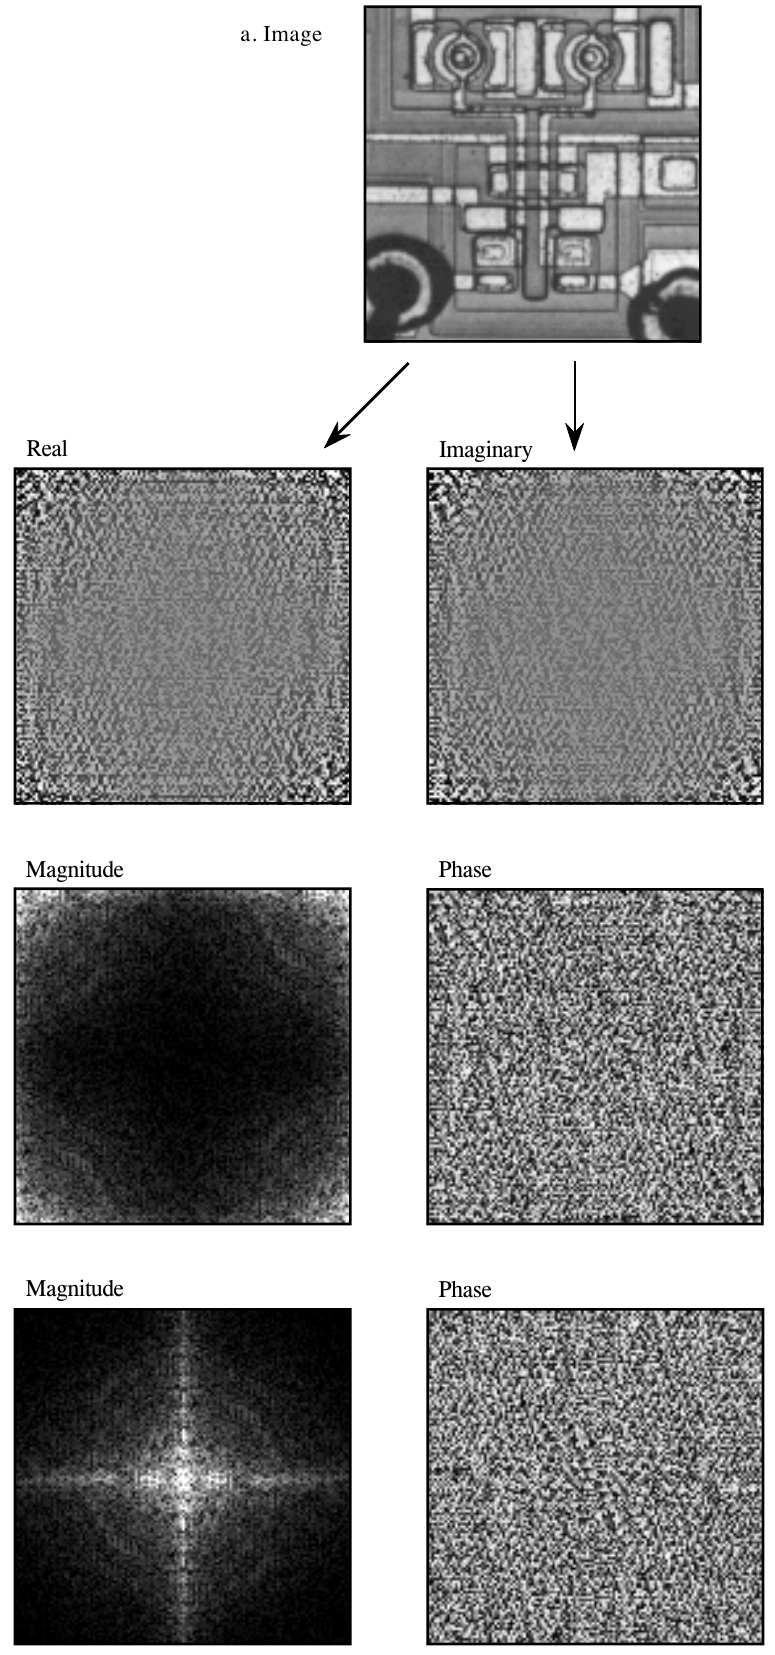
\includegraphics[width=0.646\linewidth,height=0.8\textheight,keepaspectratio]{assets/ch24/fig24-09.png}
\caption*{\textbf{图 24-9　图像的频谱。} 示例图像 (a)
是集成电路硅表面的显微照片。频谱可以显示为实部和虚部，如 (b)
所示；也可以显示为幅度和相位，如 (c) 所示。(b) 和 (c)
的显示方式是低频在四角、高频在中心。由于频域是周期的，显示可以重新排列，把这两个位置对调。这就是
(d)，其中幅度和相位以低频在中心、高频在四角的方式显示。 （从上到下：a.
Image = 图像；b. 以直角坐标形式（实部和虚部）显示的频谱，Real =
实部，Imaginary =
虚部；c.~以极坐标形式（幅度和相位）显示的频谱，Magnitude = 幅度，Phase =
相位；d.~以极坐标形式显示、并平移使零频率位于中心的频谱。原书 (b)～(d)
的说明排在各行左侧，已去掉，译文见上。）}
\end{figure}

图 24-10 说明了二维频域是怎样组织的（低频放在四角）。第 N/2 行和第 N/2
列把频谱分成四个象限。对实部和幅度来说，右上象限是左下象限的镜像，左上象限是右下象限的镜像。虚部和相位也有这种对称性，只是镜像像素的值符号相反。换句话说，频谱中每个点都有一个匹配点，对称地位于图像中心（第
N/2 行、第 N/2
列）的另一侧。其中一个点是正频率，另一个是匹配的负频率，这在第 10
章讨论一维信号时讲过。写成公式，这种对称性是：

\textbf{公式
24-2}　二维频域的对称性。这些公式对两种格式都适用：低频显示在四角时，以及通过平移把低频放到中心时。在极坐标形式下，幅度与实部有相同的对称性，相位与虚部有相同的对称性。

\[\mathrm{Re}\,X[r,c] = \mathrm{Re}\,X[N-r,\,N-c]\]

\[\mathrm{Im}\,X[r,c] = -\,\mathrm{Im}\,X[N-r,\,N-c]\]

这些公式考虑了频谱是周期的，每 N 个采样重复一次，下标从 0 到
N−1。换句话说，X{[}r, N{]} 应理解为 X{[}r, 0{]}，X{[}N, c{]} 应理解为
X{[}0, c{]}，X{[}N, N{]} 应理解为 X{[}0,
0{]}。这种对称性使频谱中有四个点与自身匹配，它们位于 {[}0, 0{]}、{[}0,
N/2{]}、{[}N/2, 0{]} 和 {[}N/2, N/2{]}。

频域中的每一对点对应空间域中的一个正弦波。如 (a) 所示，{[}0, 0{]}
处的值对应空间域中零频率的正弦波，即图像的直流分量。图中只画了一个点，因为这是与自身匹配的点之一。如
(b)、(c)、(d)
所示，其他各对点对应的二维正弦波看起来像海面上的波浪。一维正弦波有频率、相位和幅度；二维正弦波还有方向。

每个正弦波的频率和方向由这对点在频域中的位置决定。如图所示，从每个点向它所在象限外角上的零频率位置画一条线，即
{[}0, 0{]}、{[}0, N/2{]}、{[}N/2, 0{]} 或 {[}N/2,
N/2{]}（图中用圆圈标出）。这条线的方向决定空间正弦波的方向，长度与波的频率成正比。这样，低频就位于四角附近，高频位于中心附近。

\begin{figure}[htbp]
\centering
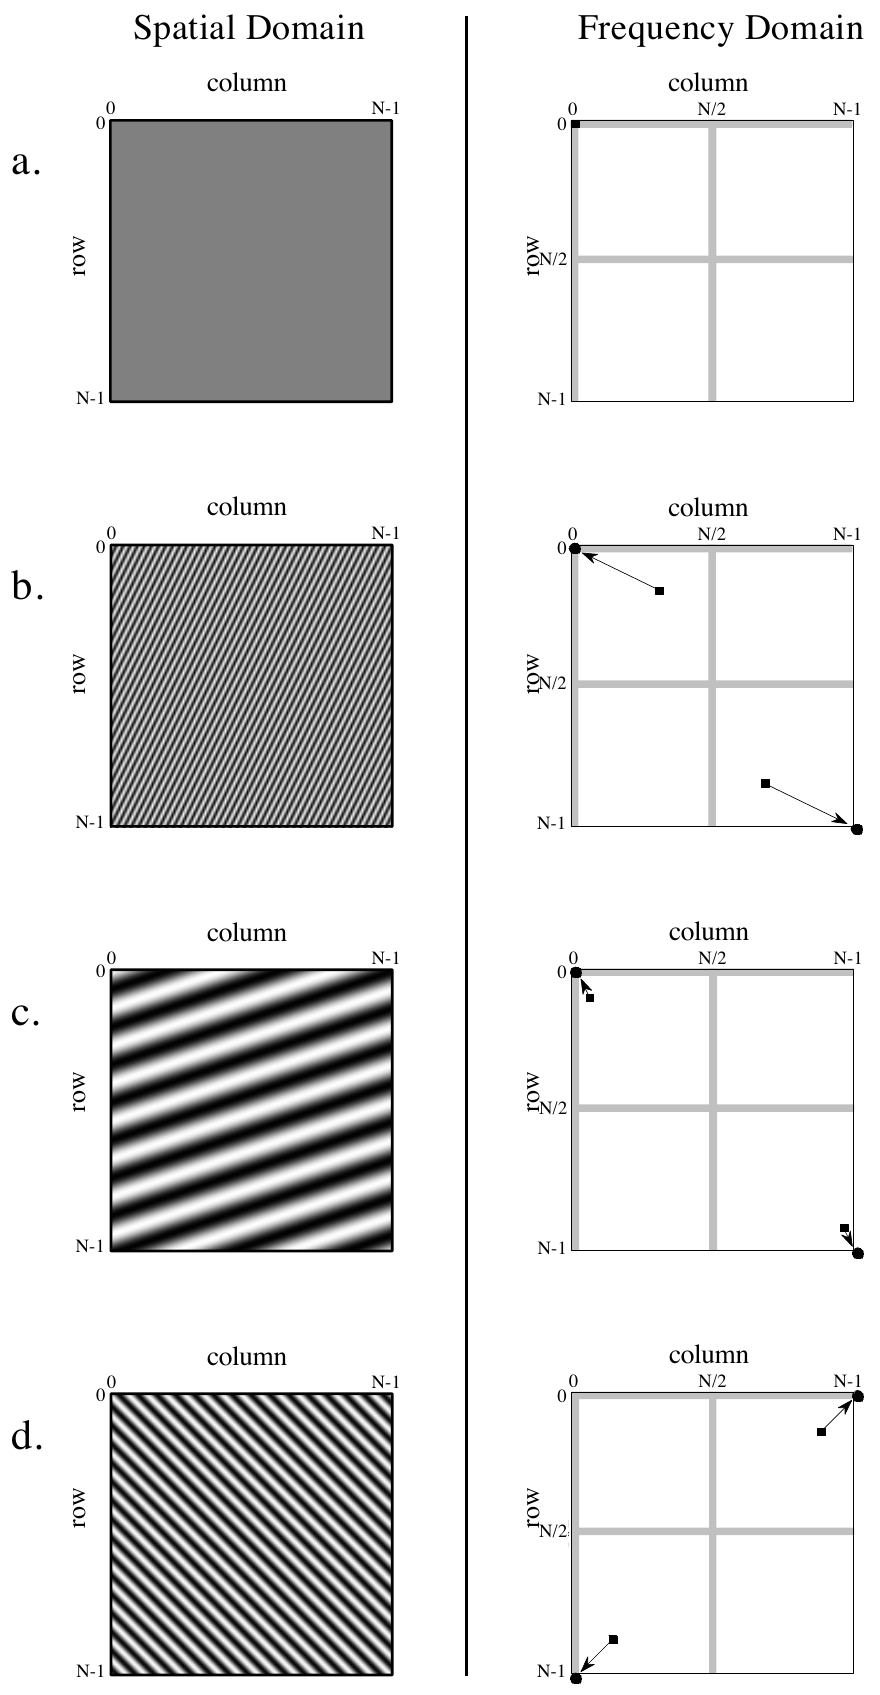
\includegraphics[width=0.733\linewidth,height=0.8\textheight,keepaspectratio]{assets/ch24/fig24-10.png}
\caption*{\textbf{图 24-10　二维正弦波。}
图像中的正弦波和余弦波既有频率又有方向。这里给出了四个例子。这些频谱以低频在四角的方式显示。频谱中的圆圈表示零频率的位置。
（Spatial Domain = 空间域，Frequency Domain = 频域；row = 行，column =
列。原书图注排在左侧，已去掉，译文见上。）}
\end{figure}

当频谱以零频率在中心的方式显示时（图
24-9d），每对点的连线都画到图像中心的直流值，即 {[}N/2,
N/2{]}。这种组织方式更容易理解和使用，因为所有的线都画到同一个点。把零放在中心的另一个好处是它与连续图像的频谱一致。空间域连续时，频域是非周期的，零频率在中心，频率向各个方向越来越高，直到无穷。一般来说，只要是给人看的场合------教科书、期刊文章、算法文档------离散图像的频谱都以零频率在中心的方式显示。然而，大多数计算是在计算机数组以另一种格式（低频在四角）存放数据的情况下进行的，因为
FFT 用的就是这种格式。

即使有了
FFT，计算傅里叶变换所需的时间仍是图像处理中的一大瓶颈。例如，在个人计算机上，一幅
512×512 图像的傅里叶变换需要几分钟。这比实时图像处理（每秒 30
帧）所需的速度大约慢 10,000
倍。执行时间这么长，是因为图像包含海量信息。打个比方，一幅典型图像中的像素数，和本书的字数差不多。随着计算机越来越快，通过频域做图像处理会越来越流行。这是一项二十一世纪的技术，看着它崛起吧！

\section{FFT 卷积}

尽管傅里叶变换很慢，它仍然是把图像与大滤波器核卷积的最快方法。例如，把一幅
512×512 的图像与一个 50×50 的 PSF 卷积，用 FFT 比常规卷积快大约 20
倍。第 18 章讨论了 FFT
卷积对一维信号是怎样工作的，二维版本是它的简单推广。

我们用一个例子来演示 FFT
卷积：在图像中定位一个预定图案的算法。假设我们要做一个检查一美元钞票的系统，可能用于印刷质量控制、伪钞检测或自动售货机的付款验证。如图
24-11 所示，采集钞票的一幅 100×100
像素的图像，以乔治·华盛顿的肖像为中心。目标是在这幅图像中搜索一个已知图案，本例中是
29×29
像素的脸部图像。问题是：给定一幅采集到的图像和一个已知图案，确定这个图案出现在图像中何处（或是否出现）的最有效方法是什么？如果你认真读过第
6 章，就知道这个问题的解是相关（匹配滤波器），而且可以用卷积来实现。

\begin{quote}
\textbf{译注：} 相关与匹配滤波在第 7
章（``相关''一节）讲过，原书此处写成第 6 章。
\end{quote}

\begin{figure}[htbp]
\centering
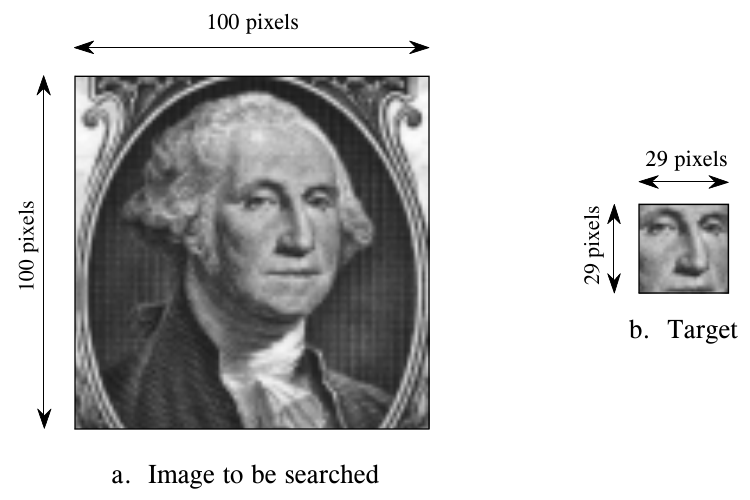
\includegraphics[width=0.625\linewidth,height=0.8\textheight,keepaspectratio]{assets/ch24/fig24-11.png}
\caption*{\textbf{图 24-11　目标检测的例子。} 问题是在 100×100
像素的乔治·华盛顿图像 (a) 中，搜索目标图案 (b)，即 29×29
像素的脸。最优解是相关，它可以通过卷积来实现。 （a. Image to be searched
= 被搜索的图像；b. Target = 目标；100 pixels = 100 像素，29 pixels = 29
像素。）}
\end{figure}

在真正做卷积之前，需要做两处修改，把目标图像变成 PSF，如图 24-12
所示。(a) 是目标信号，即我们要检测的图案。(b) 中图像被旋转了
180°，相当于先左右翻转再上下翻转。第 7
章讲过，用卷积实现相关时，目标信号需要翻转，以抵消卷积过程中发生的翻转。我们稍后会回到这个问题。

第二处修改是提高算法效果的一个技巧。与其在原图像中检测脸，不如在原图像的边缘中检测脸的边缘，这样更有效。这是因为边缘比原来的特征更锐利，使相关的峰更尖。这一步不是必需的，但能让结果明显变好。最简单的做法是，在做相关之前，对原图像和目标信号都施加一个
3×3
边缘检测滤波器。根据卷积的结合律，这等同于对目标信号施加两次边缘检测滤波器，而原图像不动。实际上，只施加一次
3×3 边缘检测核通常就够了。图 24-12 中 (b) 就是这样变成 (c) 的。这样 (c)
就是卷积要用的 PSF。

\begin{figure}[htbp]
\centering
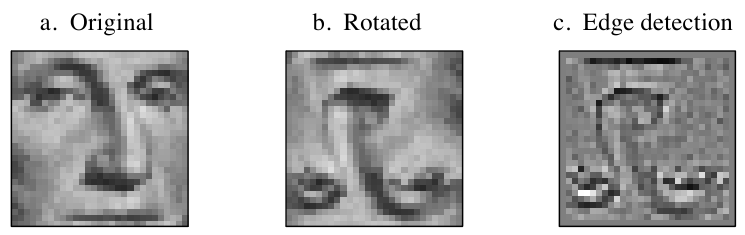
\includegraphics[width=0.621\linewidth,height=0.8\textheight,keepaspectratio]{assets/ch24/fig24-12.png}
\caption*{\textbf{图 24-12　构造相关滤波器核。} (a) 是目标信号。(b) 中把它旋转
180°，以抵消卷积中固有的翻转，从而实现相关。施加边缘检测滤波器后得到
(c)，即本例所用的滤波器核。 （a. Original = 原始；b. Rotated =
旋转后；c.~Edge detection = 边缘检测后。）}
\end{figure}

图 24-13 说明了 FFT 卷积的细节。本例中，我们把图像 (a) 与图像 (b)
卷积，得到图像
(c)。这两幅图像是为实现相关而选取和预处理过的，这一点在这里无关紧要；这是一张卷积的流程图。第一步是给两个参与卷积的信号补足够多的零，使它们的尺寸是
2 的幂，并且大到能容纳最终图像。例如，100×100 和 29×29
像素的图像卷积，所得图像是 128×128 像素。因此必须给 (a) 和 (b)
补足够的零，使它们都变成 128×128
像素。不这样做的话，就会发生圆周卷积(circular
convolution)，最终图像会失真。如果你理解这些概念有困难，回头复习第 18
章，那里对一维情形讨论得更详细。

用 FFT 算法把 (a) 和 (b) 变换到频域，得到四个 128×128
的数组，即两幅参与卷积的图像的实部和虚部。把 (a) 的实部和虚部与 (b)
的实部和虚部相乘，就得到 (c) 的实部和虚部。（如果需要回忆怎么做，见公式
9-1。）最后做逆 FFT，得到最终的卷积图像，算法完成。

\begin{figure}[htbp]
\centering
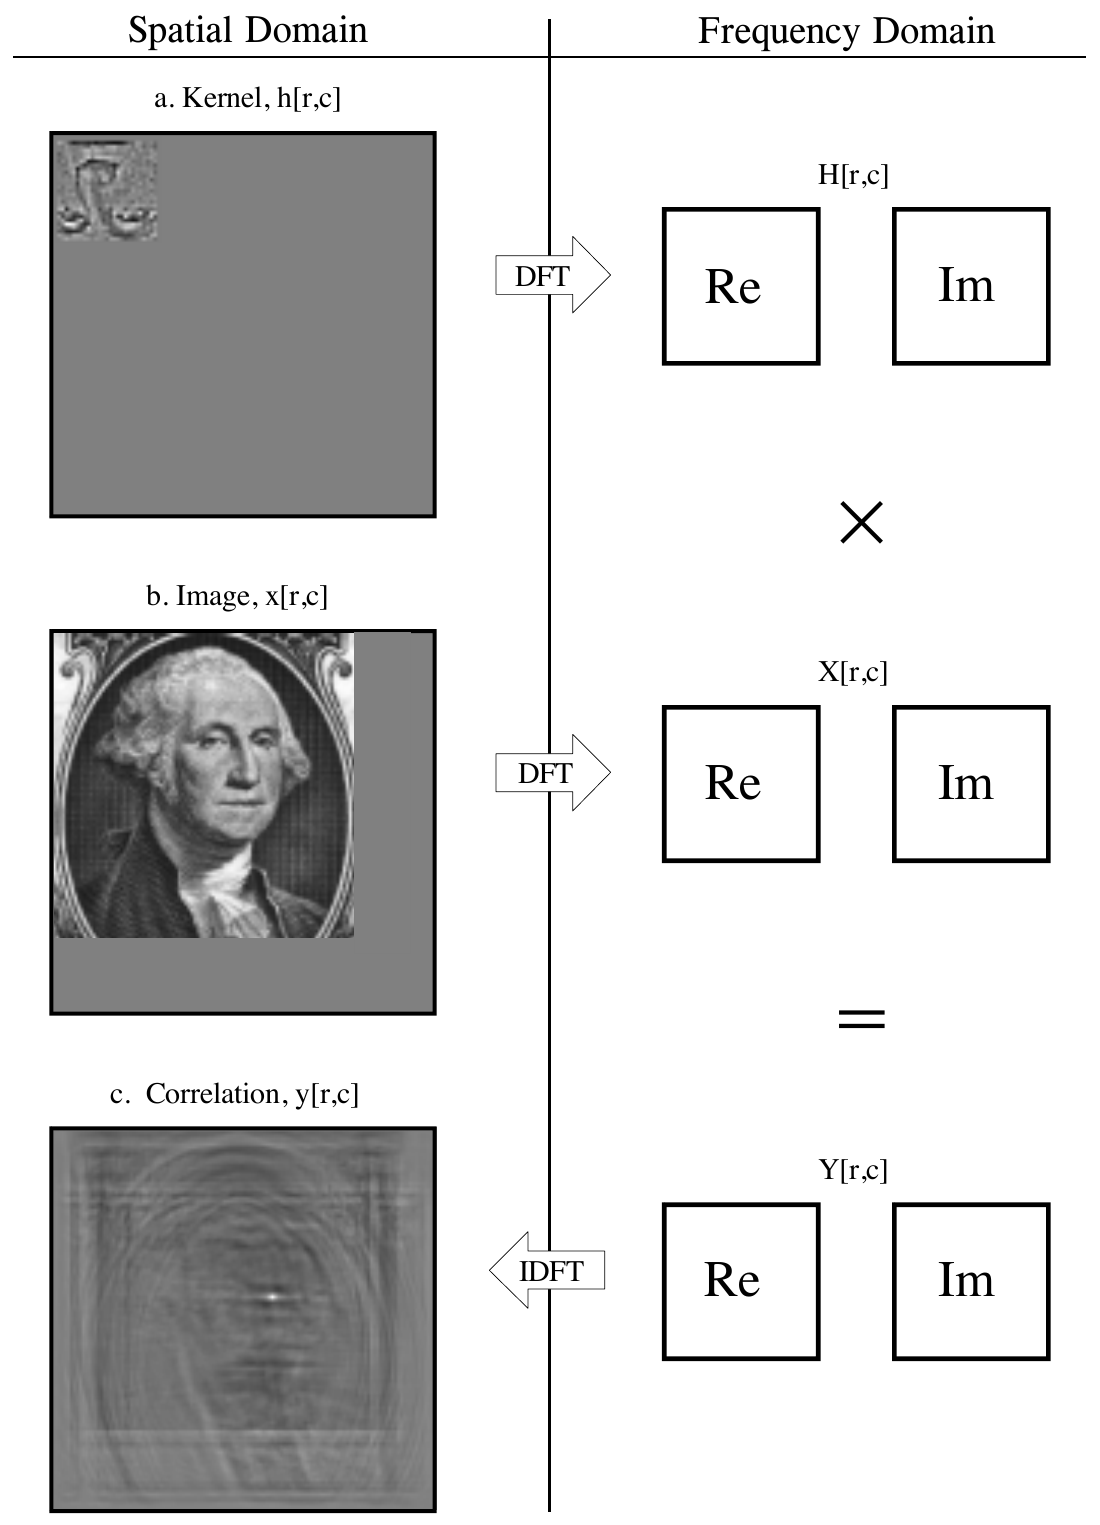
\includegraphics[width=0.917\linewidth,height=0.8\textheight,keepaspectratio]{assets/ch24/fig24-13.png}
\caption*{\textbf{图 24-13　FFT 图像卷积的流程图。} 用 FFT 把 (a) 和 (b)
中的图像变换到频域，两个频谱相乘，再用逆 FFT
回到空间域。本例中，原图像是为了通过卷积实现相关而选取和预处理过的。
（Spatial Domain = 空间域，Frequency Domain = 频域；a. Kernel,
h{[}r,c{]} = 核；b. Image, x{[}r,c{]} = 图像；c.~Correlation, y{[}r,c{]}
= 相关结果；Re = 实部，Im = 虚部；DFT / IDFT = 正变换 / 逆变换。注意图中
(a) 是核、(b) 是图像，与正文''把图像 (a) 与图像 (b)
卷积''的字母顺序不同，卷积可交换，不影响结果。）}
\end{figure}

相关图像中每个像素的值，衡量的是目标图像与被搜索图像在该点匹配得有多好。在这个例子里，相关图像
(c)
由噪声加一个明亮的峰组成，表明与目标信号匹配得很好。只要找出这幅图像中最亮的像素，就能确定检测到的脸的坐标。如果没有对目标信号做边缘检测修改，峰仍然存在，但会模糊得多。

相关虽然是图像处理中的强大工具，却有一个重大局限：目标图像必须与被搜索图像中对应区域的大小和旋转方向完全相同。噪声和各像素幅度的其他变化相对不重要，但空间上的精确匹配至关重要。例如，这使该方法几乎无法用于在军事侦察照片中寻找敌方坦克、在医学图像中寻找肿瘤、在机场行李扫描中寻找手枪。一种办法是把图像与各种形状和旋转角度的目标图像多次相关。原理上可行，但执行时间会让你很快失去兴趣。

\section{细看图像卷积}

我们用上一个例子来更详细地探讨二维卷积。和一维信号一样，图像卷积可以从输入端或输出端来看。回想第
6
章，输入端视角最能说明卷积是怎样起作用的，而输出端视角是大多数数学和算法的写法。这两种看待这个运算的方式你都需要习惯。

图 24-14
是图像卷积的输入端描述。输入图像中的每个像素都使一个经过缩放和平移的 PSF
被加到输出图像上，输出图像就是所有这些贡献的 PSF
之和。这张图展示的是输入图像中 {[}r, c{]} 位置的点对输出图像的贡献。PSF
被平移，使 PSF 中的 {[}0, 0{]} 像素对准输出图像中的 {[}r, c{]}
像素。如果 PSF 只用正下标定义（如本例），平移后的 PSF 就整个位于 {[}r,
c{]} 的右下方。别被这张图里倒过来的脸搞糊涂了：这张倒脸就是本例所用的
PSF（图 24-13a）。在输入端视角中，PSF 没有旋转，只是平移。

\begin{figure}[htbp]
\centering
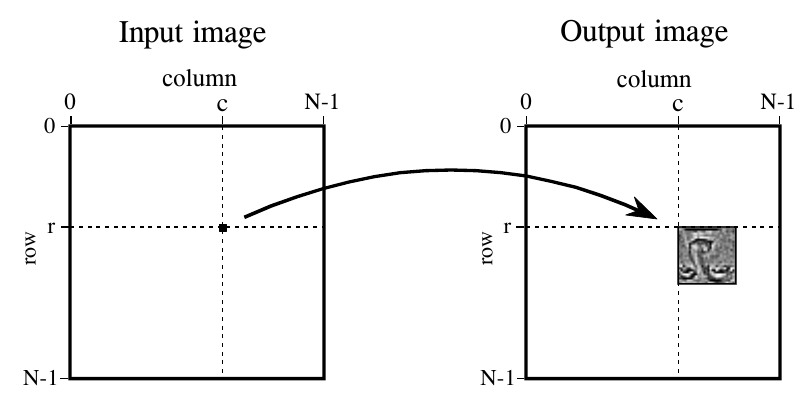
\includegraphics[width=0.667\linewidth,height=0.8\textheight,keepaspectratio]{assets/ch24/fig24-14.png}
\caption*{\textbf{图 24-14　从输入端看图像卷积。}
输入图像中的每个像素都向输出图像贡献一个经过缩放和平移的
PSF，输出图像就是这些贡献之和。图中的脸是倒的，因为这就是我们所用的
PSF。 （Input image = 输入图像，Output image = 输出图像；row =
行，column = 列。）}
\end{figure}

图 24-15 说明了从输出端看的图像卷积。输出图像中的每个像素，比如 {[}r,
c{]} 处的采样，都从输入图像的许多像素接收贡献。PSF 绕 {[}0, 0{]}
像素旋转 180°，再平移使 PSF 中的 {[}0, 0{]} 像素对准输入图像中的 {[}r,
c{]} 像素。如果 PSF 只用正下标，它就位于输入图像中 {[}r, c{]}
像素的左上方。输出图像中 {[}r, c{]} 像素的值，是把旋转后的 PSF
中的像素与输入图像中对应的像素相乘再求和得到的。这个过程由公式 24-3 和表
24-1 的程序给出。

\textbf{公式 24-3}　图像卷积。图像 x{[} , {]} 和 h{[} , {]} 卷积得到图像
y{[} , {]}。h{[} , {]} 的大小是 M×M 像素，下标从 0 到
M−1。在这个公式中，输出图像的单个像素 y{[}r, c{]} 按输出端视角计算。下标
j 和 k 用来遍历 h{[} , {]} 的行和列，计算乘积之和。

\[y[r,c] = \sum_{k=0}^{M-1} \sum_{j=0}^{M-1} h[k,j]\; x[r-k,\, c-j]\]

注意，卷积导致的 PSF 旋转抵消了设计 PSF 时所做的旋转。这使图 24-15
中的脸是正的，与输入图像中要检测的图案方向相同。也就是说，我们成功地用卷积实现了相关。对比图
24-13c 和图 24-15，就能看出相关图像中的亮点是怎样表示检测到了目标的。

\begin{figure}[htbp]
\centering
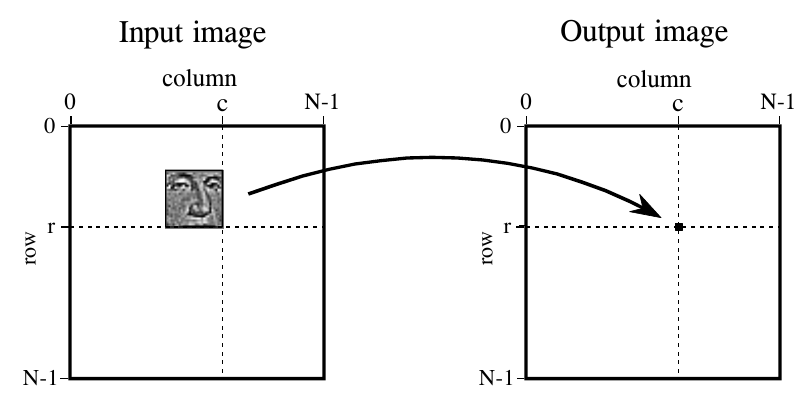
\includegraphics[width=0.667\linewidth,height=0.8\textheight,keepaspectratio]{assets/ch24/fig24-15.png}
\caption*{\textbf{图 24-15　从输出端看图像卷积。}
输出信号中的每个像素，等于旋转后的 PSF
中的像素与输入图像中对应像素的乘积之和。 （Input image =
输入图像，Output image = 输出图像；row = 行，column = 列。）}
\end{figure}

FFT 卷积给出的输出图像，与表 24-1 的常规卷积程序相同。FFT
卷积缩短的执行时间，真的值得增加的程序复杂度吗？我们仔细看看。图 24-16
比较了三种方法的执行时间：用浮点数的常规卷积（标为
FP）、用整数的常规卷积（标为 INT）和用浮点数的 FFT 卷积（标为
FFT）。给出了两种图像尺寸的数据：512×512 和 128×128。

\textbf{表 24-1}　常规图像卷积（注释已译成中文）。

\begin{Shaded}
\begin{Highlighting}[]
\NormalTok{100 CONVENTIONAL IMAGE CONVOLUTION}
\NormalTok{110 \textquotesingle{}}
\NormalTok{120 DIM X[99,99]             \textquotesingle{}存放输入图像，100×100 像素}
\NormalTok{130 DIM H[28,28]             \textquotesingle{}存放滤波器核，29×29 像素}
\NormalTok{140 DIM Y[127,127]           \textquotesingle{}存放输出图像，128×128 像素}
\NormalTok{150 \textquotesingle{}}
\NormalTok{160 FOR R\% = 0 TO 127        \textquotesingle{}遍历输出图像的每一行和每一列，}
\NormalTok{170 FOR C\% = 0 TO 127        \textquotesingle{}按公式 24{-}3 计算像素值}
\NormalTok{180 \textquotesingle{}}
\NormalTok{190   Y[R\%,C\%] = 0           \textquotesingle{}把这个像素清零，用作累加器}
\NormalTok{200 \textquotesingle{}}
\NormalTok{210   FOR J\% = 0 TO 28       \textquotesingle{}把核中的每个像素与输入图像中对应的像素相乘，}
\NormalTok{220   FOR K\% = 0 TO 28       \textquotesingle{}再加到累加器上}
\NormalTok{230     Y[R\%,C\%] = Y[R\%,C\%] + H[J\%,K\%] * X[R\%{-}J\%,C\%{-}J\%]}
\NormalTok{240   NEXT K\%}
\NormalTok{250   NEXT J\%}
\NormalTok{260 \textquotesingle{}}
\NormalTok{270 NEXT C\%}
\NormalTok{280 NEXT R\%}
\NormalTok{290 \textquotesingle{}}
\NormalTok{300 END}
\end{Highlighting}
\end{Shaded}

\begin{quote}
\textbf{译注：} 第 230 行的 \texttt{X{[}R\%-J\%,C\%-J\%{]}}
是笔误，按公式 24-3 列下标应为 \texttt{C\%-K\%}。另外，程序没有检查
\texttt{R\%-J\%}、\texttt{C\%-K\%} 是否落在输入图像的 0～99
范围内，照原样运行会越界；第 6 章表 6-2 用 \texttt{IF\ ...\ GOTO}
跳过越界项，这里也应如此。C 版本对这两处都做了修正。
\end{quote}

\textbf{C 实现}（完整可编译版本见
\texttt{c/table24-1\_image\_convolution.c}，其中还实现了 FFT
卷积和可分离卷积，用来对照验证）：

\begin{Shaded}
\begin{Highlighting}[]
\CommentTok{/* 常规卷积：公式 24{-}3 的直接实现，从输出端逐像素计算 */}
\DataTypeTok{static} \DataTypeTok{void}\NormalTok{ convolve\_direct}\OperatorTok{(}\DataTypeTok{double}\NormalTok{ y}\OperatorTok{[}\NormalTok{NY}\OperatorTok{][}\NormalTok{NY}\OperatorTok{])}
\OperatorTok{\{}
    \ControlFlowTok{for} \OperatorTok{(}\DataTypeTok{int}\NormalTok{ r }\OperatorTok{=} \DecValTok{0}\OperatorTok{;}\NormalTok{ r }\OperatorTok{\textless{}}\NormalTok{ NY}\OperatorTok{;}\NormalTok{ r}\OperatorTok{++)}            \CommentTok{/* 160：遍历输出的每一行 */}
        \ControlFlowTok{for} \OperatorTok{(}\DataTypeTok{int}\NormalTok{ c }\OperatorTok{=} \DecValTok{0}\OperatorTok{;}\NormalTok{ c }\OperatorTok{\textless{}}\NormalTok{ NY}\OperatorTok{;}\NormalTok{ c}\OperatorTok{++)} \OperatorTok{\{}      \CommentTok{/* 170：遍历输出的每一列 */}
            \DataTypeTok{double}\NormalTok{ acc }\OperatorTok{=} \FloatTok{0.0}\OperatorTok{;}               \CommentTok{/* 190：累加器清零 */}
            \ControlFlowTok{for} \OperatorTok{(}\DataTypeTok{int}\NormalTok{ j }\OperatorTok{=} \DecValTok{0}\OperatorTok{;}\NormalTok{ j }\OperatorTok{\textless{}}\NormalTok{ NH}\OperatorTok{;}\NormalTok{ j}\OperatorTok{++)}    \CommentTok{/* 210：遍历核的每一行 */}
                \ControlFlowTok{for} \OperatorTok{(}\DataTypeTok{int}\NormalTok{ k }\OperatorTok{=} \DecValTok{0}\OperatorTok{;}\NormalTok{ k }\OperatorTok{\textless{}}\NormalTok{ NH}\OperatorTok{;}\NormalTok{ k}\OperatorTok{++)} \OperatorTok{\{}  \CommentTok{/* 220：遍历核的每一列 */}
                    \DataTypeTok{int}\NormalTok{ rr }\OperatorTok{=}\NormalTok{ r }\OperatorTok{{-}}\NormalTok{ j}\OperatorTok{,}\NormalTok{ cc }\OperatorTok{=}\NormalTok{ c }\OperatorTok{{-}}\NormalTok{ k}\OperatorTok{;}
                    \ControlFlowTok{if} \OperatorTok{(}\NormalTok{rr }\OperatorTok{\textless{}} \DecValTok{0} \OperatorTok{||}\NormalTok{ rr }\OperatorTok{\textgreater{}=}\NormalTok{ NX }\OperatorTok{||}\NormalTok{ cc }\OperatorTok{\textless{}} \DecValTok{0} \OperatorTok{||}\NormalTok{ cc }\OperatorTok{\textgreater{}=}\NormalTok{ NX}\OperatorTok{)} \ControlFlowTok{continue}\OperatorTok{;}  \CommentTok{/* 原书缺的越界检查 */}
\NormalTok{                    acc }\OperatorTok{+=}\NormalTok{ H}\OperatorTok{[}\NormalTok{j}\OperatorTok{][}\NormalTok{k}\OperatorTok{]} \OperatorTok{*}\NormalTok{ X}\OperatorTok{[}\NormalTok{rr}\OperatorTok{][}\NormalTok{cc}\OperatorTok{];}  \CommentTok{/* 230：原书误印为 X[R\%{-}J\%,C\%{-}J\%] */}
                \OperatorTok{\}}
\NormalTok{            y}\OperatorTok{[}\NormalTok{r}\OperatorTok{][}\NormalTok{c}\OperatorTok{]} \OperatorTok{=}\NormalTok{ acc}\OperatorTok{;}
        \OperatorTok{\}}
\OperatorTok{\}}
\end{Highlighting}
\end{Shaded}

运行结果（在这台机器上实测）： - \textbf{测试 1，常规卷积 vs FFT 卷积：}
100×100 图像与 29×29 核，FFT 卷积补零到 128×128，两者 128×128
个输出像素的最大偏差为 7.8e-14，说明 FFT
卷积给出的输出图像与常规卷积相同。耗时：常规卷积约 17 ms，FFT 卷积约 4
ms。 - \textbf{测试 2，用卷积实现相关：} 在含噪的 100×100 图像第 40
行、第 55 列处埋一个 29×29 的不对称图案，把图案旋转 180°
作为核去卷积，输出的最亮点恰好落在 {[}68,
83{]}，即图案在输入中的位置加上核的尺寸 28，检测正确。 - \textbf{测试
3，可分离卷积：} 29×29
的高斯核拆成两个一维投影，先卷行再卷列，与直接二维卷积的最大偏差为
1.1e-13；耗时从约 17 ms 降到约 0.6 ms。

首先注意，FFT 卷积所需的执行时间与核的大小无关，因此图中是平直的线。在
100 MHz 奔腾个人计算机上，用 FFT 卷积处理一幅 128×128 的图像大约需要 15
秒，而 512×512 的图像需要 4 分多钟。把计算次数加起来可以看出，对 N×N
的图像，FFT 卷积的执行时间与 \(N^2\log_2 N\) 成正比。也就是说，512×512
的图像所需时间约为 128×128 图像的 20 倍。

\begin{figure}[htbp]
\centering
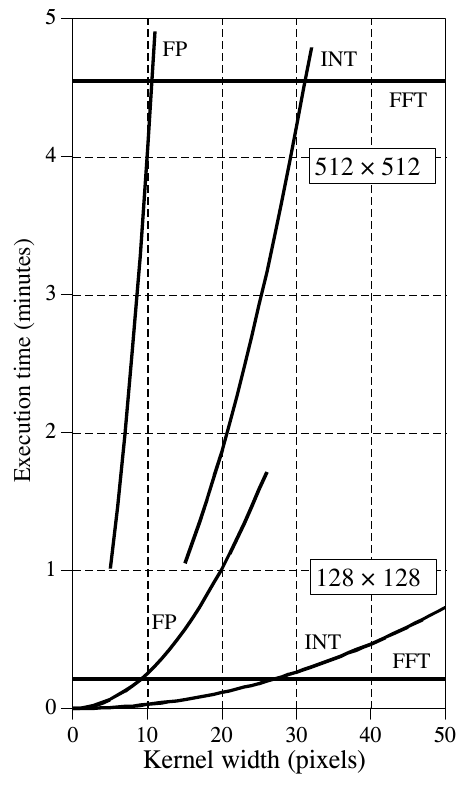
\includegraphics[width=0.388\linewidth,height=0.8\textheight,keepaspectratio]{assets/ch24/fig24-16.png}
\caption*{\textbf{图 24-16　图像卷积的执行时间。} 这张图给出了在 100 MHz
奔腾处理器上三种图像卷积方法的执行时间：用浮点运算的常规卷积
(FP)、用整数的常规卷积 (INT)，以及用浮点数的 FFT 卷积
(FFT)。两组曲线分别对应 512×512 和 128×128 像素的输入图像。使用 FFT
卷积时，时间只取决于图像大小，与核的大小无关。相比之下，常规卷积既取决于图像大小，也取决于核的大小。
（Execution time (minutes) = 执行时间（分钟），Kernel width (pixels) =
核宽度（像素）。原书图注排在左侧，已去掉，译文见上。）}
\end{figure}

对 N×N 的图像与 M×M 的核卷积，常规卷积的执行时间与 \(N^2M^2\)
成正比。看看表 24-1
的程序就能明白这一点。换句话说，常规卷积的执行时间强烈依赖于所用核的大小。如图所示，核大于约
10×10 像素时，FFT
卷积比用浮点数的常规卷积快。大多数情况下，常规卷积可以用整数，这使盈亏平衡点提高到约
30×30
像素。如图所示，这些盈亏平衡点略微依赖于被卷积图像的大小。要记住的概念是：FFT
卷积只对大滤波器核有用。
